Hier wird die Variante des Deep Cascade vorgestellt. 
Die Deep Cascade Netze werden iterativ während dem Training aufgebaut. Es bleibt dabei ein einziges Netz. Es wird zuerst 
definiert, welcher Optimizer und welcher Loss in dem Netz genutzt wird. 

\begin{figure}[htpb]
    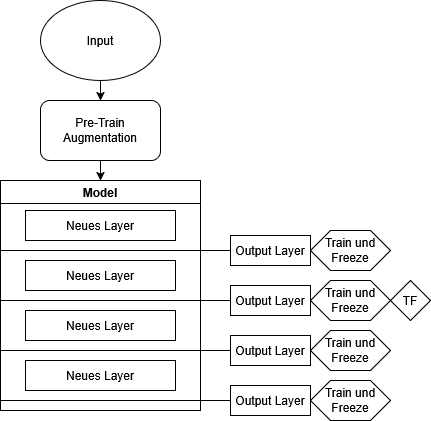
\includegraphics[height=10cm]{../../Graphiken/deepcascade_2.png}
    \caption{\label{fig:deepcascade} Vorstellung Deep Cascade Aufbau}
\end{figure}

Sobald dies beides gemacht wurde, wird im Netz das Erste Layer definiert. Dieses wird ergänzt durch ein Output Layer und dann trainiert. 
Wenn das Training beendet wird, wird das Output Layer gelöscht und ein neues Layer hinzugefügt, wie es in Figure 2.1 gezeigt wird. Zudem wird 
das gerade trainierte Layer gefreezt, damit dieses keine weiteren Aktualisierungen mehr bekommt. 
Dann wiederholt sich das Training, das löschen, das freezing und weitere hinzufügen von Layern. 
An einer beliebigen Stelle kann TF gemacht werden, indem, statt in der Trainingsphase den Sourcedatensatz zu nutzen, der Targetdatensatz 
genutzt wird. 

% Sollte ich nicht vorher Kaskadierung erklären? Oder geht das hier? Hier könnte ich auch Graphen bauen. Ist glaube ich sogar besser, wenn 
% ich es tue...
